\section*{Appendix: A spatial-curvature tensor distinguishes equal-scalar initial data}
The scalar spatial curvature in an instantaneous energy constraint does
not determine the full intrinsic curvature. To display the missing
information, choose an oriented right-handed orthonormal triad,
\(\epsilon_{123}=+1\), signature \((-+++ )\), and

\begin{equation}
K_{ij}=-(h\delta_{ij}+S_{ij}),\qquad h=H/c,\quad S=\sigma/c,
 \qquad \kappa_g=8\pi G/c^4.\tag{A1}
\end{equation}

The symmetric structure tensor \(n\) and vector \(a\) satisfy \(na=0\).
The signed momentum and Hamiltonian constraints in this convention are

\begin{equation}
\kappa_g q_i=3S_{ij}a_j+\epsilon_{ijk}n_{jl}S_{kl},\qquad
 3h^2=\kappa_g\varepsilon_N+\Lambda+\tfrac12S:S-\tfrac12{}^{(3)}R.\tag{A2}
\end{equation}

Here \(\varepsilon_N\) and \(q\) are normal-frame energy-density and
flux-density coordinates in J/m\^{}3; the corresponding energy current
is \(cq\). The quantities \(n,a,h,S\) have inverse-length units. In the
class-A subspace \(a=0\), the spatial Ricci tensor is

\begin{equation}
{}^{(3)}\!\mathrm{Ric}
 =2n^2-(\operatorname{tr}n)n+
 [\tfrac12(\operatorname{tr}n)^2-\operatorname{tr}(n^2)]I.\tag{A3}
\end{equation}

This tensor formula supplies a finite map independent of a photon
transfer calculation.

Set \(u_*=10^{-26}\,\mathrm{m}^{-1}\), \(h/u_*=2\),
\(S/u_*=\operatorname{diag}(1/10,-1/20,-1/20)\), and \(\Lambda=0\). The
choices \(n/u_*=\operatorname{diag}(1,0,0)\) and
\(n/u_*=\operatorname{diag}(0,2,1)\) provide type-II and unequal
type-VII\(_0\) witness presentations. Both have \begin{equation}
{}^{(3)}R/u_*^2=-1/2,\qquad
 \kappa_g\varepsilon_N/u_*^2=4697/400,\qquad q=0,\tag{A4}
\end{equation} while their ordered Ricci spectra are \((-1/2,-1/2,1/2)u_*^2\) and
\((-3/2,-1/2,3/2)u_*^2\). The minimum Frobenius separation of their
proper-rotation orbits is \(\sqrt2\,u_*^2\). Equal scalar curvature and
the displayed common matter/expansion/shear coordinates therefore leave
different intrinsic curvature tensors.

For a finite uncertainty calculation, use the 12 dimensionless
coordinates consisting of the six Frobenius coordinates of \(n/u_*\),
\(h/u_*\), and five signed STF coordinates of \(S/u_*\). The map \(F\)
returns six Ricci coordinates, normal energy and three signed flux
coordinates, all normalized by \(u_*^2\) with \(\kappa_g\) for matter.
Each input set is \(z=z_0+L\xi\), \(\|\xi\|\le1\), with
\(L=\operatorname{diag}(0.05,\ldots,0.05,0.01,\ldots,0.01)\), seven
entries followed by five. This is a declared deterministic ellipsoid,
not a covariance estimate. Since this map is quadratic,

\begin{equation}
F(z_0+L\xi)=F(z_0)+JL\xi+\tfrac12\mathcal H[L\xi,L\xi].\tag{A5}
\end{equation}

For a projection \(w\), a whole-set radius is \begin{equation}
b_w=\|L^TJ^Tw\|_2+\tfrac12\|L^T\mathcal H_wL\|_{\rm op}
 +e_{\rm round},\qquad \mathcal H_w=\sum_k w_k\mathcal H_k.\tag{A6}
\end{equation}

The sum of conservative Ricci Frobenius radii for the two matched sets
is \(0.41697619\,u_*^2\), below their orbit-center separation. Thus
these two constructed tensor sets are disjoint under the stated bound.
Their neighborhoods need not retain the center's Bianchi class or a
common perfect-fluid model. Positivity bounds establish \(h>0\) and
\(\varepsilon_N>0\) throughout these sets, while signed flux can vary.

\begin{table}[htbp]
\centering\small
\caption{Center coordinates normalized by $u_*$ for $n,h,S$ and $u_*^2$ for $\kappa_g\varepsilon_N,\kappa_gq$. Diagonal tuples display the complete diagonal center tensors; all off-diagonal entries and $a$ vanish. Ranks refer to geometry and joint maps.}\label{tab:geo}
\begin{tabular}{llllllll}
\toprule
Center & $\mathrm{diag}\,n$ & $h$ & $\mathrm{diag}\,S$ & $\kappa_g\varepsilon_N$ & $\kappa_gq$ & Geom. & Joint \\
\midrule
II & (1,0,0) & 2 & (0.1,-0.05,-0.05) & 11.7425 & (0,0,0) & 6 & 9 \\
VII0matched & (0,2,1) & 2 & (0.1,-0.05,-0.05) & 11.7425 & (0,0,0) & 6 & 10 \\
I & (0,0,0) & 2 & (0,0,0) & 12.0000 & (0,0,0) & 0 & 1 \\
flatVII0 & (0,1,1) & 2 & (0,0,0) & 12.0000 & (0,0,0) & 3 & 6 \\
\bottomrule
\end{tabular}
\end{table}

The two flat controls use \(n=0\) and
\(n/u_*=\operatorname{diag}(0,1,1)\), both with \(S=0\), \(h/u_*=2\),
\(\kappa_g\varepsilon_N/u_*^2=12\), and \(q=0\). Both have zero full
spatial Riemann and the same local Euclidean intrinsic geometry through
distinct simply transitive presentations. At II, unequal VII\(_0\), I
and flat VII\(_0\), the six-component geometry Jacobian ranks are 6, 6,
0 and 3; the ten-component joint-image ranks are 9, 10, 1 and 6. At type
I only the first energy derivative is nonzero,
\(\partial(\kappa_g\varepsilon_N/u_*^2)/\partial(h/u_*)=12\). A zero
geometry Jacobian does not make the map constant:
\(\mathrm{Ric}(tn)=t^2\mathrm{Ric}(n)\). The nonzero Hessian and curved
exactly flat paths must be retained when interpreting the local rank.

\begin{figure}[htbp]
\centering
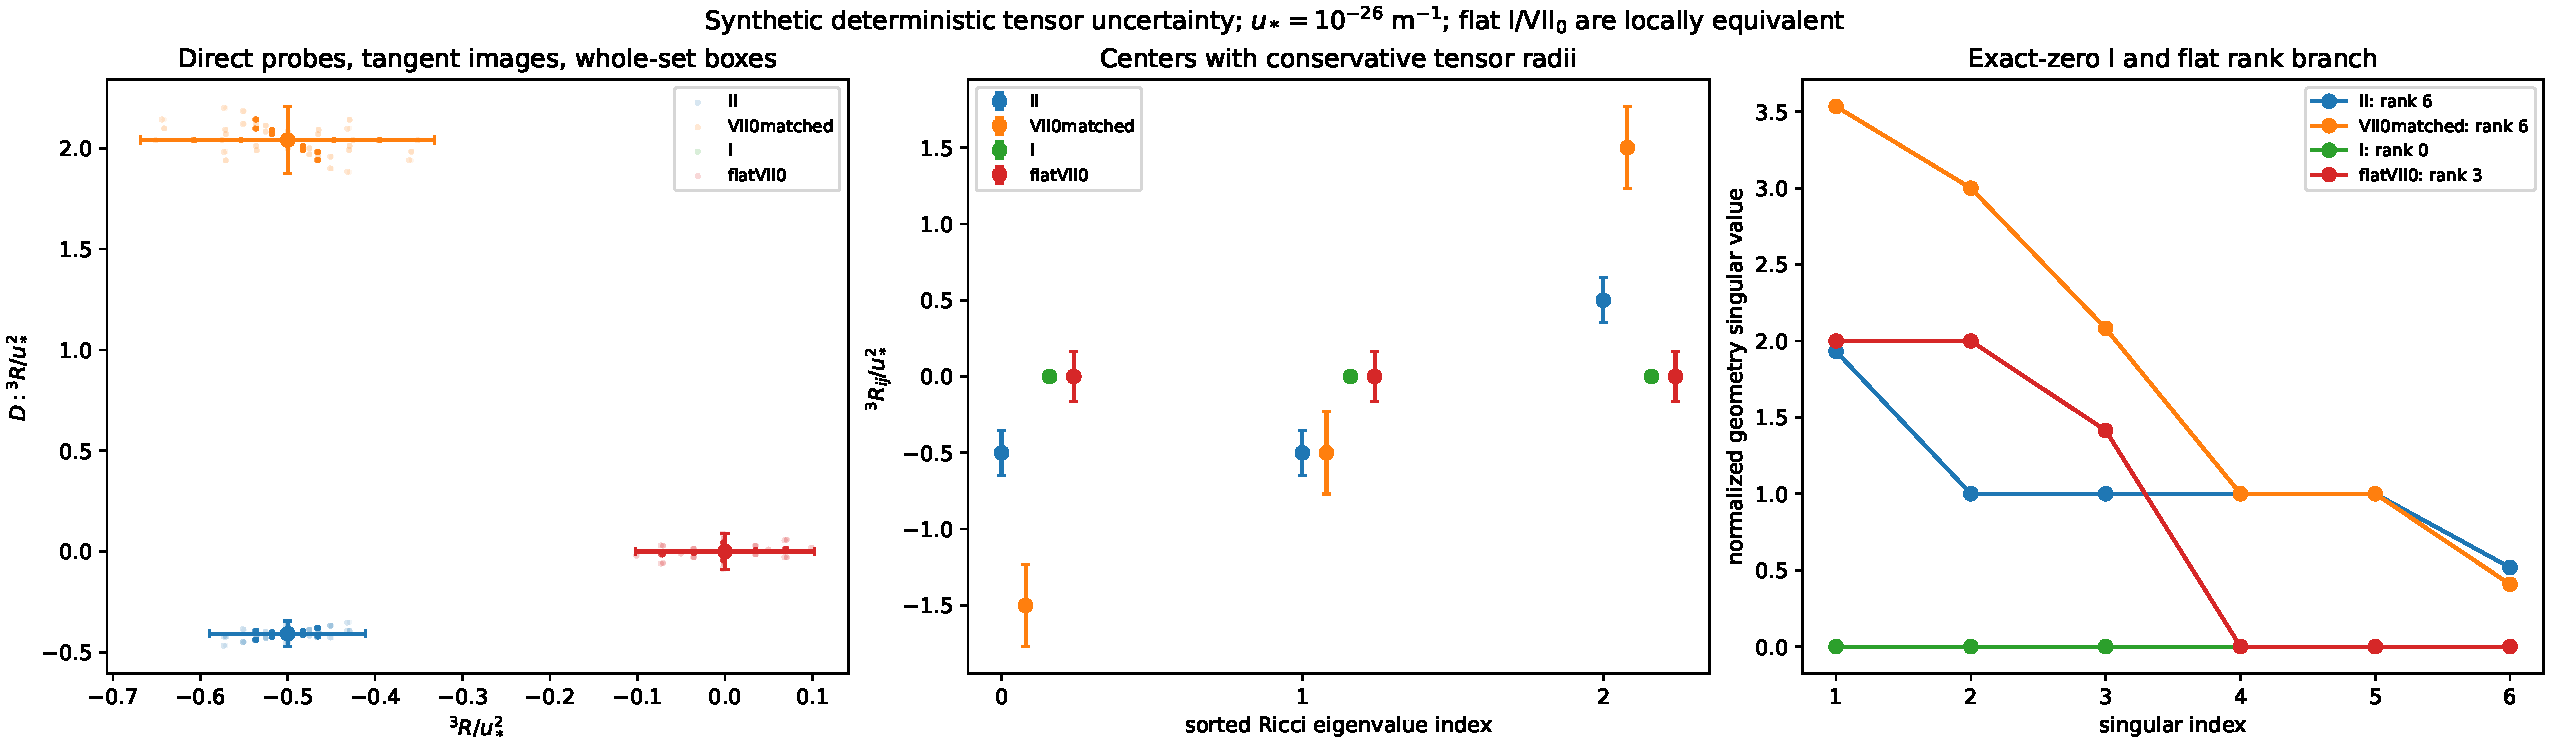
\includegraphics[width=0.95\linewidth]{r36_geometry/geometry_image.pdf}
\caption{Deterministic images of four declared initial-data ellipsoids. Left: 577 prescribed probes per center and conservative whole-set bounds in scalar and tensor projections. Middle: center Ricci spectra and conservative tensor radii. Right: singular values of the six-component geometry Jacobian, not the ten-component joint map. Probe clouds visualize the sets; the whole-set quadratic enclosure establishes the stated separation. Center labels name witness presentations, and the two flat centers describe the same local intrinsic Euclidean geometry. No empirical probability or coverage is assigned.}
\end{figure}

The connection to the LRS-V region studied in the main text preserves
all 280 retained tensor tuples. The proper cyclic frame transformation
\((e_1,e_2,e_3)=(e_z,e_x,e_y)\) carries signed shear, flux, pressure and
anisotropic stress into this triad. The retained maximum relative
Hamiltonian and momentum residuals are \(1.11\times10^{-16}\) and
\(9.48\times10^{-17}\). Velocity remains the physical speed
\(\beta=v/c\), with matter velocity undefined in the absent-matter
vacuum branch. This algebraic conversion is not an evolved spacetime
solution or a measured curvature constraint. An observational use
requires a calibrated, same-frame response to the curvature tensor.
Neither scalar agreement nor tensor-set separation identifies a Bianchi
family from a CMB sky.
